L'étude pilote s'est déroulée en 2 temps distincts. Le premier temps suivait un protocole clair tandis que le deuxième prenait la forme d'un atelier de découverte et de co-création
lors duquel on travaillait main dans la main avec les acteurs afin de répondre à leurs envies et leurs besoins particuliers. 

Le déroulé de la première étape fut le suivant: 
\begin{itemize}
    \item Phase préalable: les comédiens reçoivent le monologue à travailler chez eux afin d'apprendre le texte uniquement (on ne leur demande pas de faire un travaille d'étude à proprement parler ou ils chercheraient à incarner au mieux le personnage)
    \item Phase d'introduction:  Les participants sont accueillis et informés des détails de l'expérience à laquelle ils vont prendre part. On leur explique que leur objectif, dans chaque environnement virtuel qu’ils exploreront, sera d’utiliser la liberté d’action qui leur est offerte, s’ils en ont, pour créer un cadre dans lequel ils se sentiront le plus immergés dans le personnage qu’ils incarnent, un environnement qui leur permet de jouer et de donner du sens au texte qu'ils jouent. 
    \item Phase d'immersion: chaque participant va alors faire une suite de 6 immersions différentes au cours des 2 premiers jours de l'étude
    \begin{itemize}
    \item Phase d'adaptation: Le participant peut alors mettre le casque. Il sera d'abord en immersion dans une salle vide et sobre qui lui permettra de faire une transition fluide avec le monde virtuel et qui lui permettra de s'approprier l'espace et les différentes commandes (la téléportation et les menus de modifications de l'environnement)
    \item Phase d'exploration et de création de l'environnement: Dans le cas où l'environnement lui est entièrement imposé, le comédien va tout de même avoir un temps d'exploration de celui-ci avant de commencer à jouer afin de se l'approprier, de s'y sentir à l'aise et de choisir son emplacement et son orientation de jeu. Dans le cas où il peut le construire et le modifier, cette phase va se découper en deux temps. Lors du premier il va pouvoir moduler son environnement autant qu'il le souhaite et une fois l'environnement bloqué, il pourra faire la même phase d'exploration pour se retrouver dans l'espace créer avant de commencer à jouer.
    
    \item Phase de jeu en réalité virtuelle: Le comédien joue son monologue en immersion dans le casque de réalité virtuelle.
    \item Phase de questionnaire: Afin d'éviter les biais liés à la transition entre le monde virtuel et le monde réel dans l'auto-évaluation des expériences en réalité virtuelle \cite{Alexandrovsky}, une partie des retours (en particulier le questionnaire de présence) se font en immersion dans une salle vide une fois le jeu du comédien terminé. 
    \item Phase de retours: Une fois l'immersion terminée, nous avons échangé de façon informelle avec les comédiens afin de noter leurs retours d'experience pour chacun des environnements et chacunes des modalités de modification de ces derniers. 
    \end{itemize}
    \item Phase de jeu au plateau: Une fois les 6 expériences terminées, le comédien joue une fois son monologue au plateau, en dehors du casque de VR, afin de voir si les immersions qu'il a vécues ont une influence, si certaines images vues lui reviennent naturellement pendant son jeu et si oui lesquelles ont été les plus marquantes et les plus créatrices de jeu. 
\end{itemize}

\begin{figure}[h]
    \centering

    \begin{minipage}[b]{0.31\textwidth}
        \centering
        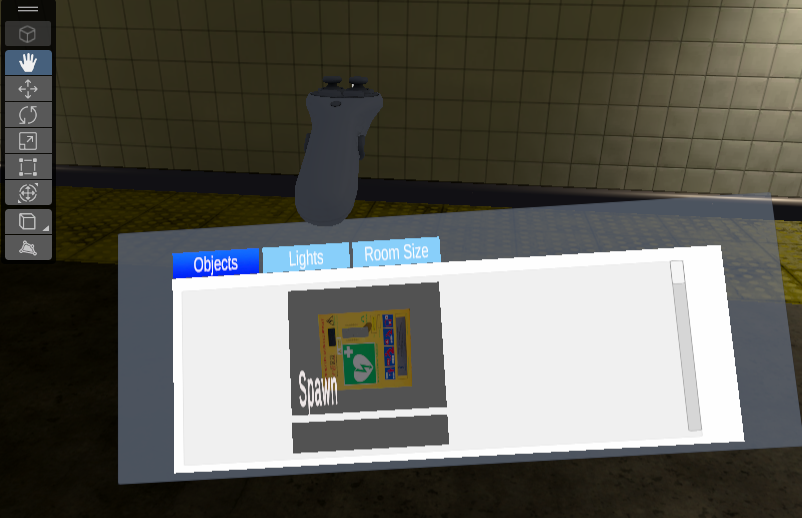
\includegraphics[width=\textwidth]{images/subwayhandmenu.png}
    \end{minipage}
    \hfill
    \begin{minipage}[b]{0.345\textwidth}
        \centering
        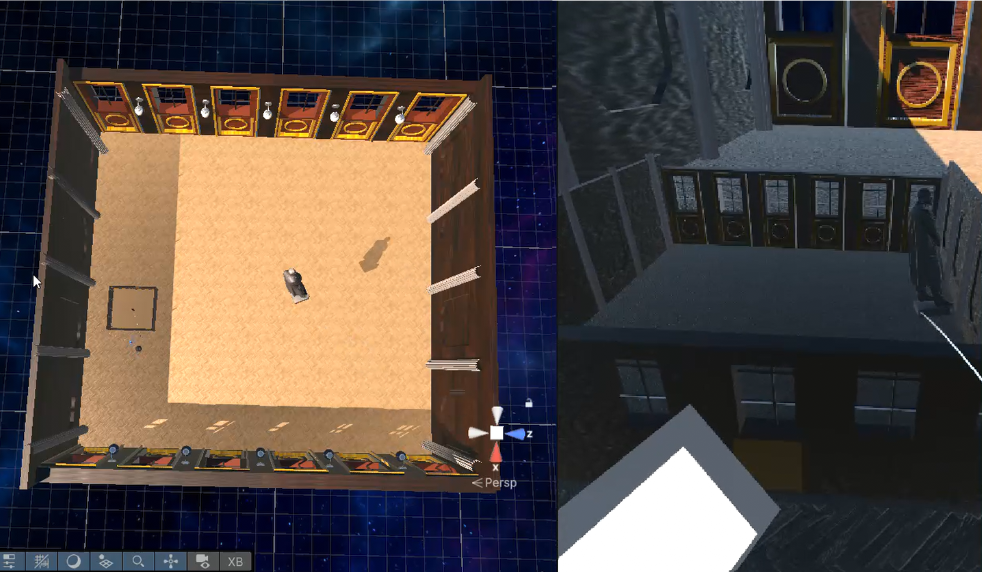
\includegraphics[width=\textwidth]{images/amphihandmenu.png}
    \end{minipage}
    \hfill
    \begin{minipage}[b]{0.32\textwidth}
        \centering
        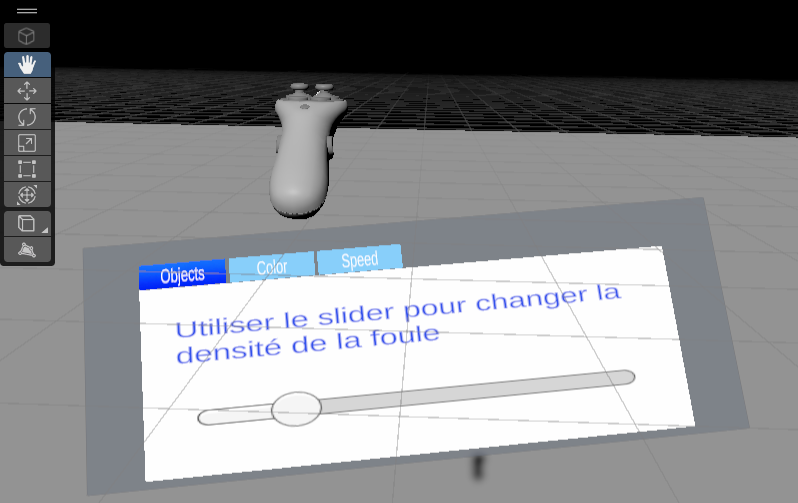
\includegraphics[width=\textwidth]{images/foghandmenu.png}
    \end{minipage}

  \caption{Captures d'écran des 3 modalités de modification des environnements (de gauche à droite: menu permettant de modifier la taille, la luminsoté et de placer des nouveaux objets dans l'environnement scénographique, outil de placement des objets dans une maquette à petite échelle dans l'environnement narratif, menu permettant de modifier la densité de la foule, la couleur et la vitesse du brouillard dans l'environnement abstrait)}
  \label{fig:trois_images}
\end{figure}


